\documentclass[11pt]{article}
\usepackage{a4wide}
\usepackage[T3,T1]{fontenc}
\usepackage[noenc]{tipa}
\usepackage{tipx}
\usepackage[notipa]{ucs}
\usepackage[utf8x]{inputenc}
\usepackage[english,UKenglish]{babel}
\def \thiscode {en}
\input{dxIOL11en}
\newcommand \dmy [3]{#1/#2/#3} %%% UK, IE, OZ
\newcommand \dialog {dialogue}
\newcommand \axe {axe}
\renewcommand \airplane {aeroplane}
\newcommand \ous {ou$_{\textrm{\small sg}}$}
\newcommand \oup {ou$_{\textrm{\small pl}}$}
%%% from http://tex.stackexchange.com/questions/26870/check-if-a-string-contains-a-given-character
\makeatletter
\def\instring#1#2{TT\fi\begingroup
  \edef\x{\endgroup\noexpand\in@{#1}{#2}}\x\ifin@}
\makeatother
\newcommand \anintern [1]{a\if\instring{#1}{aeiou}n\fi\ #1}
\newcommand \aninterm {\expandafter \anintern }
\newcommand \an {\expandafter \expandafter \expandafter \aninterm }
%\addtolength{\oddsidemargin}{-.875in}
%\addtolength{\evensidemargin}{-.875in}
%\addtolength{\topmargin}{-.525in}
%\addtolength{\textwidth}{1.75in}
%\addtolength{\textheight}{1.4in}
%\usepackage{colortbl}
\usepackage{graphicx}

\newenvironment{assgts}{%
\renewcommand \labelenumi {\bfseries \zagrad {\alph {enumi}}}%
\renewcommand \labelenumii {\arabic {enumii}.}%
\begin{enumerate}}{\end{enumerate}}

\newcommand \by [1]{%
  \unskip\nobreak\hfil\penalty50
  \hbox{}\nobreak\hfill{\hbox{\qquad\itshape #1}}\par}
\newcommand \byx [1]{%
  \unskip\nobreak\hfil\penalty50
  \hbox{}\nobreak\hfill{\hbox{\qquad #1}}\par}
%\newcommand \book[1]{{\slshape #1\/}}
\newcommand \bord [1]{{\fontencoding{T1}\bfseries\itshape\selectfont #1\/}}
\newcommand \word [1]{{\itshape #1\/}}
\newcommand \ipaword [1]{[\ipa{#1}]}
\newcommand \ipa [1]{\bgroup#1\egroup}
\newcommand \bipa [1]{\bgroup\bfseries#1\egroup}
\let \super \textsuperscript
\newcommand \synt [1]{\L{\textsf{#1}}}
\newcommand \tallstrut {\vrule height 9pt depth 0pt width 0pt}
\newcommand \deepstrut {\vrule height 0pt depth 2pt width 0pt}
\newcommand \placehold {\fbox{\fbox{\quad} \fbox{\quad} \fbox{\quad}}}
\def \hh {\textsuperscript h}
%\let \visiblespace \textvisiblespace
\newcommand \latehta [1]{\quoted{#1\space}}
\newlength\halftext
\halftext=\textwidth \advance \halftext by-50pt \divide \halftext by2
\newcommand \NB {{\ooalign{\hfil\raise.2ex\hbox{\bfseries!}\hfil\crcr\Large$\bigtriangleup$}}}
\ifx \upcase \undefined \newcommand \upcase [1]{\MakeUppercase {#1}}\fi
\newcommand \Upcase {\expandafter \upcase }
\newcommand \Uppcase {\expandafter \expandafter \expandafter \Upcase }
\ifx \locase \undefined \newcommand \locase [1]{\MakeLowercase {#1}}\fi
\newcommand \Locase {\expandafter \locase }
\newcommand \Lowcase {\expandafter \expandafter \expandafter \Locase }
\ifx \zagrat \undefined \newcommand \zagrat [1]{\zagrad{#1.}}\fi
%\newcommand \upsens [2]{\MakeUppercase {#1#2}}
%\newcommand \thead {\expandafter \upsens }
%\let \thead \relax
\mathchardef\nga="223A

\def \1#1(#2,#3){\if #10#2\else #3\fi}
\def \3#1(#2,#3:#4/#5/#6){\if #10#2\else #3\ifcase #1\relax \or #4\or #5\or #6\fi\fi}
\def \9#1(#2,#3:#4/#5/#6){\if #10#2\else #3\ifcase #1\relax \or #4\or #5\or #5\or #6\fi\fi}
\def \4#1(#2,#3:#4/#5/#6/#7){\if #10#2\else #3\ifcase #1\relax \or #4\or #5\or #6\or #7\fi\fi}
\def \proper #1{\underline {\Upcase #1}}

%\def \Stress {ˈ}
%\def \Strett {ˈˈ}
\def \Stress {$^1$}
\def \Strett {$_2$}

\makeatletter
\def \ps@firstpage {
\let\@oddfoot\@empty
\def\@oddhead{\hfill \Huge \bf \thiscode}}
\def \ps@somestyle {
\let\@oddfoot\@empty
\def\@oddhead{\ifx \N \relax
\textsl {\small \begin{tabular}[t]{@{}l}\nthIOL {\thisth}\ \zagrad{\N{2013}}.\\ \chapname \end{tabular}}\hfill \thepage
\else \thepage \hfill
\textsl {\small \begin{tabular}[t]{r@{}}\R{\nthIOL {\thisth}\ \zagrad{\N{2013}}.}\\ \R{\chapname} \end{tabular}}
\fi }}
%\def \procherk {\hrulefill}
\def \procherk {\leaders \hbox {:}\hfill \kern\z@}
\newcommand{\Rom}[1]{\expandafter\@slowromancap\romannumeral #1@}
\makeatother

\newcounter {exx}[section]
\newcounter {ex:bundiny}
\ifx \N \undefined
  \let \N \relax
  \let \R \relax
  \let \L \relax
  \newcommand \zagrad [1]{(#1)}
  \def \lr {l}\def \bimapp {rll}
  \newcommand \biline [2]{\addtocounter{exx}{1}\arabic{exx}. & #1 & #2}
  \newcommand \ciline [3]{\addtocounter{exx}{1}\arabic{exx}. & \multicolumn{2}{l}{(#1?)} \\ & #3 & #2.}
  \newcommand \bidyir [2]{\addtocounter{exx}{1}\arabic{exx}. & \bord{#1.} \\& #2.}
  \newcommand \biriyd [2]{\addtocounter{exx}{1}\arabic{exx}. & #1. \\& \bord{#2.}}
  \newcommand \squoted [1]{‘#1’}
\else
  \renewcommand \bord [1]{\L{\bfseries\itshape\selectfont #1\/}}
  \renewcommand \bipa [1]{\L{\bgroup\fontencoding{T3}\bfseries\selectfont\SetUnicodeOption{tipa}#1\egroup}}
  \newcommand \zagrad [1]{)#1(}
  \def \lr {r}\def \bimapp {lrl}
  \newcommand \biline [2]{#2 & \R{#1} & \addtocounter{exx}{1}.\arabic{exx}}
  \newcommand \ciline [3]{&\hfill \R{)#1?(} & \addtocounter{exx}{1}.\arabic{exx}\\ \R{#2.} & #3}
  \newcommand \bidyir [2]{\bord{#1.} & \addtocounter{exx}{1}.\arabic{exx}\\\hfill \R{#2.}}
  \newcommand \biriyd [2]{\hfill \R{#1.} & \addtocounter{exx}{1}.\arabic{exx}\\\bord{#2.}}
  \newcommand \squoted [1]{\L{'}#1\L{`}}
\fi
\ifx \zagrad \undefined \fi
\ifx \postpar \undefined \newcommand \postpar {.}\fi
\newcommand \paaS [2]{\bord{#1 paa #2.}}

\newcommand \georow [3]{#1. & \R{#3} & \ipa{[#2]}}

\def \problem {\stepcounter {section}\paragraph{\probword \thesection\ \zagrad{\N{20} \pontword}\postpar }}
\def \solution {\stepcounter {section}\paragraph{\probword \thesection \postpar }}

\newcommand \makepart [1]{\newpage
\thispagestyle{firstpage}
  \begin{center}%
  {\LARGE \nthIOL {\thisth} \par }
  \vskip 1em{\Large
  \thistown\ \zagrad {\thisland}, \mbox{\olydates {22}{26}{\Julyname}{2013}}
  \par }
%  \vskip 1em{\begin{tabular}[t]{c}\Large
%  \thistown\ (\thisland), \olydates {30}{\Julyname}{3}{\Auguname}{2012}
%  \end{tabular}\par }
  \vskip 1em{\large #1}\end{center}\par \vskip .5em
  \def \chapname {#1}\setcounter {section}0\setcounter {page}1}

\begin{document}
\ifx\enumLat\undefined\else\enumLat\fi

\makepart{\probplur {\indicont}}

\pagestyle{somestyle}

%\centerline{\textbf{\regulats}}
%
\regulado. \regulare. \regulami. \towarrant.

\regulaty. \regulatz.\bigskip

\hrule

\problem \givemots {\inthelg {\Yidiny}} \andtrans {\tothislang}:\medskip \\
%
\centerline{\begin{tabular}{l\ifx \N \relax l\else r\fi}
\bipa{guda:ga} & \galika 1\\
\bipa{buɲa} & \bunya 1\\
\bipa{wagu:ɟa} & \Man 1\\
\bipa{muyubara} & \muyubara 1\\
\bipa{gaɟagimba:gu} & \ggu {\gajagimba}\\
\bipa{bamagimbal} & \gimbal {\bama}\\
\bipa{bama:gu} & \ggu {\bama}\\
\bipa{bimbi:bi} & \alter {\bimbi}\\
\bipa{mularigu} & \ggu {\mulari}\\
\bipa{mularini} & \nnigen {\mulari}\\
\bipa{buɲa:m} & \mmu {\bunya}\\
\end{tabular}\hfill
\begin{tabular}{l\ifx \N \relax l\else r\fi}
\bipa{gudagabi} & \alter {\galika}\\
\bipa{gaɟagimba:m} & \mmu {\gajagimba}\\
\bipa{biɲɟi:ngu} & \ggu {\binyjin}\\
\bipa{bimbi:n} & \nnigen {\bimbi}\\
\bipa{muɟam} & \mujam 1\\
\bipa{biɲɟi:nmu} & \mmu {\binyjin}\\
\bipa{maɟu:rbi} & \alter {\majur}\\
\bipa{buɲagimbal} & \gimbal {\bunya}\\
\bipa{baɟigalni} & \nnigen {\bajigal}\\
\bipa{ɟudu:lumuɟay} & \mujay {\judulu}\\
\end{tabular}}\medskip \\
%
\hetteken {\quoted{\bipa :}}\ \marpslen.
%
\begin{assgts}
\item \marklong\ (\ifthEany):
\begin{tabular}{l\ifx \N \relax l\else r\fi}
\bipa{mugaɽumu} & \mmu {\mugaRu}\\
\bipa{waŋalgu} & \ggu {\waval}\\
\end{tabular}
\item \marklong\ (\ifthEany) \et {\Locase \fordinto {\tothislang}}:

\centerline{\bipa{baman}, \bipa{buɲabi}, \bipa{maɟurmuɟay}, \bipa{muɟamni}.}
\item \fordinto {\tolg {\Yidiny}}:

\centerline{\nnigen {\muyubara}, \ggu {\mugaRu}, \bimbi 1, \mmu {\majur},}
\centerline{\gimbal {\Man}, \nnigen {\judulu}, \bajigal 1, \gimbal {\waval}.}
\end{assgts}
%
\NB \quad \infamily {\Thelg {\Yidiny}}{\toPNyfam}. \spokenca{150}{\inQueend}.
%
\bipa{ɟ, ŋ, ɲ, ɽ} \aconsons.
%
\by{—\BBname, \IDname}	

\newpage

\problem \givemots {\inTundra {\Yukaghir}} \andtrans {\tothislang} \chaotict:
%
\begin{center}
\bord{ilennime, joqonnime, saancohoje, johudawur, ilenlegul, cireme, johul, aariinmøŋer, joqodile, møŋer, ciremennime, joqoncohoje, saadoŋoj, uoduo, oŋoj, aariinjohul, uodawur, joqol}\medskip

\aariinmyver,
\saan \saadovoj,
\johul,
\cireme,
\joqon \cohoje,
\ilenlegul,\\
\ovoj,
\aariinjohul,
\joqodile,
\johudawur,
\saan \nime,
\uoduo,\\
\myver,
\joqol,
\uodawur,
\ilennime,
\saan \cohoje,
\ciremennime
\end{center}
%
\begin{assgts}
\item \corrcorr.
\item \motmeans {\bord{ewce}}{\squoted{\ewceA, \ewceB}}.
\fordinto {\tothislang}:\medskip

\centerline{\bord{aarii, aariidoŋoj, ciremedawur, ile, johudewce, legul, saal, saannime, uo.}}
\twomsame.

\item \motmeans {\bord{cuo}}{\squoted{\cuo}}.
\fordinto {\tolgsky {\Yukaghir}}:\medskip

\centerline{\cuon \cireme, \johunmyver, \cohojedewce, \legudovoj.}
\ifnosure.
\end{assgts}
%
\NB \quad \onyukaga {\Yukaghir}. \onyukagb, \onyukagc {\Yukaghir}{(\egYakut)}.

\yohudawur.
\by{—\IDname}

\newpage

\problem \giwordss {\inthelg {\Piraha}} \et {\siscript}:\medskip\\
%
\begin{tabular}{lll}
\bord{bagiai baabi} & \ipa{ba.gia.{\Stress}baa.bi} & \bagiaibaabi \\
\bord{bahoigatoi} & \ipa{ba.hoi.ga.{\Stress}toi} & \bahoigatoi 1 \\
\bord{bahoigatoi baihiigi} & \ipa{ba.{\Strett}hoi.ga.to.bai.{\Stress}hii.gi} & \baihiigi \bahoigatoi \\
\bord{giopai} & \ipa{gio.{\Stress}pai} & \galika 1 \\
\bord{giopai hoigi} & \ipa{gio.pa.{\Stress}hoi.gi} & \hoigi \galika \\
\bord{giopai sabi} & \ipa{gio.pa.{\Stress}sa.bi} & \sabi \galika \\
\bord{giopai xaibogi} & \ipa{{\Strett}gio.pa.{\Stress}ai.bo.gi} & \xaibogi \galika \\
\bord{hixi} & \ipa{hi.{\Stress}ʔi} & \hixi 1 \\
\bord{hixi xitaixi} & \ipa{hi.ʔii.{\Stress}tai.ʔi} & \xitaixi \hixi \\
\bord{kagahoaogii toio} & \ipa{ka.ga.ho.ao.gi.to.{\Stress}io} & \toio \kagahoaogii \\
\bord{kagaihiai} & \ipa{ka.{\Stress}gai.hi.ai} & \jaguar 1 \\
\bord{kagaihiai baagiso} & \ipa{ka.gai.{\Strett}hia.{\Stress}baa.gi.so} & \baagiso \jaguar \\
\bord{kagaihiai xaibogi} & \ipa{ka.gai.{\Strett}hia.{\Stress}ai.bo.gi} & \xaibogi \jaguar \\
\bord{kagihi} & \ipa{ka.gi.{\Stress}hi} & \kagihi \\
\bord{kahai baihiigi} & \ipa{ka.{\Strett}ha.bai.{\Stress}hii.gi} & \baihiigi \kahai \\
\bord{kaibai xogiai} & \ipa{kai.{\Stress}bao.gi.ai} & \xogiai \monkey \\
\bord{kaoaibogi} & \ipa{kao.{\Stress}ai.bo.gi} & \kaoaibogi 1 \\
\bord{kaoaibogi sabi} & \ipa{kao.ai.bo.gi.{\Stress}sa.bi} & \sabi \kaoaibogi \\
\bord{koxopa} & \ipa{ko.ʔo.{\Stress}pa} & \koxopa \\
\bord{piahaogixisoaipi} & \ipa{pia.hao.gi.ʔi.so.{\Stress}ai.pi} & \piahaogixisoaipi \\
\bord{poogaihiai} & \ipa{poo.{\Stress}gai.hi.ai} & \poogaihiai 1 \\
\bord{tagasaga} & \ipa{ta.ga.{\Stress}sa.ga} & \tagasaga \\
\bord{xabagi} & \ipa{{\Stress}ʔa.ba.gi} & \xabagi 1 \\
\bord{xabagi giisai} & \ipa{ʔa.ba.gi.gii.{\Stress}sai} & \giisai\ \xabagi 1 \\
\bord{xagai} & \ipa{ʔa.{\Stress}gai} & \xagai \\
\bord{xaogii} & \ipa{{\Stress}ʔao.gii} & \xaogii \\
\bord{xibogi} & \ipa{{\Stress}ʔi.bo.gi} & \xibogi \\
\bord{xiga} & \ipa{{\Stress}ʔi.ga} & \xiga \\
\bord{xiiaapisi} & \ipa{ʔii.{\Stress}aa.pi.si} & \xiiaapisi \\
\bord{xisipoai} & \ipa{ʔi.si.po.{\Stress}ai} & \xisipoai \\
\bord{xisitai xagai} & \ipa{ʔi.si.{\Stress}taa.gai} & \xisitaixagai \\
\bord{xisoobai} & \ipa{ʔi.{\Stress}soo.bai} & \xisoobai \\
\bord{xogiai} & \ipa{ʔo.gi.{\Stress}ai} & \xogiaI \\
\end{tabular}\smallskip
%
\shortstack{
\includegraphics[bb = 0 0 260 260,scale=.4]{cartoon-toucan-11.jpg}\\{\small \xabagi 1}}\\
%
\transcri:\medskip\\
%
\begin{tabular}{ll}
\bord{xaaibi} & \xaaibi \\
\bord{xaapisi} & \xaapisi \\
\bord{xitiixisi} & \xitiixisi \\
\end{tabular}
\begin{tabular}{ll}
\bord{bigi} & \bigy  \\
\bord{kagahoaogii} & \kagahoaogii 1 \\
\bord{kaibai} & \monkey 1 \\
\bord{kapiigaiitoii} & \kapiigaiitoii \\
\end{tabular}
\begin{tabular}{ll}
\bord{poogaihiai toio} & \toio \poogaihiai \\
\bord{xabagi kapioxio} & \alter \xabagi \\
\bord{xabagi xogiai} & \xogiai \xabagi \\
\end{tabular}\medskip \\
%
\NB \quad \piragena \Piraha. \soloMura.

[\ipa{ʔ}] \isaconst\ (\glotstop).
[h] = \glotfric.
\hetteken {\quoted{\,.\,}} \syllbond.
\hetteken {\quoted{\,\ipa{\Stress}\,}} \stremark {\primary}.
\hetteken {\quoted{\,\ipa{{\Strett}}\,}} \stremark {\secondary} (\ifthEone).
%
\by{—\ASname}

\newpage

\problem \givesent {\inthelg {\Muna}} \andtrans {\tothislang}:\medskip\\
%
\mbox{}\qquad \begin{tabular}{l@{ }l}
\bidyir{murihino andoandoke dofoni we molo}{\murihino {\underline {\Upcase \demonkey}} \munazina}\\
\bidyir{lambuku nakumodoho}{\lambuku\ \nakudomoho}\\
\bidyir{lambuhindo lagahi nofanaka}{\munasubc\ \dofanaka}\\
\bidyir{lagahino damumaa kaleino robhine}{\lagahino\ \munazind}\\
\bidyir{a dhini nofumaa ndokehiku}{\dhini\ \munazine}\\
\bidyir{robhineno naghumoli lambuno adhiadhini}{\robhineno\ \munazinf}\\
\bidyir{a kontuhi namanaka}{\kontuhi\ \damanaka}\\
\bidyir{a robhinehi dakumala we andoandoke}{\robhinehi\ \munazinh}\\
\bidyir{a murihi dosuli we lambuhi}{\murihi\ \munazini}\\
\bidyir{lagahino muriku dokodoho}{\munasubj\ \dokodoho}\\
\bidyir{adhiadhini nododo molondo}{\adhiadhini\ \munazink}\\
\end{tabular}
%
\begin{assgts}
\item \fordinto {\tothislang}:
\begin{enumerate}\setcounter{enumii}{\value{exx}}
\item\bord{andoandoke nogholi lagahiku.}
\item\bord{a dhinihi dasumuli we murindo robhinehi.}
\setcounter{exx}{\value{enumii}}
\end{enumerate}
\item \fordinto {\tolg {\Muna}}:
\begin{enumerate}\setcounter{enumii}{\value{exx}}
\item \alaalaga\ \munazinl.
\item \lagahi\ \munazinm.
\item \munasubn\ \munazinn.
\item \molohino {\demonkey} \dokodoho.
\setcounter{exx}{\value{enumii}}
\end{enumerate}
\end{assgts}
%
\NB \quad \infamily {\Thelg {\Muna}}{\toAustNs}. \spokenca{300\,000}{\inInesia}.

\undernom.
%
\by{—\XGname}

\newpage

\problem \telepata {2010}{\CMUniloc\ (\villPitt, \countUSA)}. \telepatc {60}. \telepatd.

\telepate.\medskip \\
%
\begin{tabular}{|l|l|l|l|l|l|}\hline
\Upcase \wordword &\Upcase \transion &\Upcase \location A &\Upcase \location B &\Upcase \location C &\Upcase \location D\\\hline
\bord{airplane} & \airplane & \high & \low & \low & \high\\
\bord{apartment} & \apartment & \high & \low & \low & \high\\
\bord{arm} & \xaapisi & \low & \high & \low & \low\\
\bord{corn} & \corn & \low & \low & \high & \low\\
\bord{cup} & \cup & \low & \low & \high & \low\\
\bord{igloo} & \igloo & \high & \low & \low & \low\\
\bord{key} & \key & \high & \high & \low & \low\\
\bord{lettuce} & \lettuce & \low & \low & \high & \high\\
\bord{screwdriver} & \screwdriver & \low & \high & \low & \high\\ \hline
\end{tabular}\medskip \\
%
\sameinfo:
\bord{bed} \squoted{\bed},
\bord{butterfly} \squoted{\butterfly},
\bord{cat} \squoted{\cat},
\bord{cow} \squoted{\cow},
\bord{refrigerator} \squoted{\refrigerator},
\bord{spoon} \squoted{\spoon}.
\medskip \\
%
\begin{tabular}{|l|l|l|l|l|}\hline
\Upcase \wordword &\Upcase \location A &\Upcase \location B &\Upcase \location C &\Upcase \location D\\\hline
1 & \low & \low & \high & \high\\
2 & \low & \low & \high & \low\\
3 & \high & \low & \low & \low\\
4 & \low & \low & \low & \high\\
5 & \low & \high & \high & \low\\
6 & \low & \low & \low & \low\\ \hline
\end{tabular}\medskip \\
%
\corrcorr.
%(((Explain your solution))).
%
\by{—\BIname}

\bigskip

\vfill
%\hline

\begin{center}
\textbf{\editorsz:} \edinames.\medskip

\textbf{\thistext:} \whowroti.\medskip

\large \goodluck!
\end{center}

\makepart{\soluplur {\indicont}}
%\thispagestyle{empty}
\pagestyle{somestyle}
%
\solution \rulesmot:
%
\begin{enumerate}
\item \Upcase \iftotpar {\wordLoc\ (= \stemNom\ + \endingN)}{\sodo}, \allshort.
\Upcase \iftotpar {\wordLoc}{\liho}, \lgulpart.
%\begin{itemize}
%\item \iftotpar {\stemLoc}{\sodo}, \thatleng {\ultimate};
%\item \iftotpar {\stemLoc}{\liho}, \thatleng {\penultim}.
%\end{itemize}

\newcommand \odd [2]{\shortstack{#1\\\bipa #2}}
\newcommand \even [2]{\shortstack{\textbf{#1}\\\bipa{#2}}}
\hfill
\begin{tabular}{|lr@{-}l|}\hline
$2=2+0$: & \bipa{bu$_1$ɲa$^2$} & $\emptyset$\\
$4=2+2$: & \bipa{bu$_1$ɲa$^2$} & \bipa{gi$_3$mbal$^4$}\\
$4=3+1$: & \bipa{gu$_1$da$^2$ga$_3$} & \bipa{bi$^4$}\\
$4=4+0$: & \bipa{mu$_1$yu$^2$ba$_3$ra$^4$} & $\emptyset$\\
\hline
\end{tabular}
\begin{tabular}{|lr@{}l@{-}l|}\hline
$3=2+1$: & \bipa{ba$_1$\underline{ma:$^2$}} && \bipa{gu$_3$}\\
$3=3+0$: & \bipa{gu$_1$\underline{da:$^2$}} & \bipa{ga$_3$} & $\emptyset$\\
$5=3+2$: & \bipa{ɟu$_1$\underline{du:$^2$}} & \bipa{lu$_3$} & \bipa{mu$^4$ɟay$_5$}\\
$5=4+1$: & \bipa{ga$_1$ɟa$^2$gi$_3$m\underline{ba:$^4$}} && \bipa{gu$_5$}\\
\hline
\end{tabular}
\item \folloses {\bipa{-ni} \au\ \bipa{-mu}}.
\end{enumerate}
%
\begin{assgts}
\item \bipa{mugaɽumu}, \bipa{waŋa:lgu}.
\item \bipa{bama:n} — \nnigen {\bama}, \bipa{buɲa:bi} — \alter {\bunya}, \bipa{maɟurmuɟay} — \mujay {\majur}, \bipa{muɟa:mni} — \nnigen {\mujam}.
\item \nnigen {\muyubara} — \bipa{muyubara:n}, \ggu {\mugaRu} — \bipa{mugaɽugu}, \bimbi 1 — \bipa{bimbi}, \mmu {\majur} — \bipa{maɟu:rmu}, \gimbal {\Man} — \bipa{wagu:ɟagimbal}, \nnigen {\judulu} — \bipa{ɟuduluni}, \bajigal 1 — \bipa{baɟi:gal}, \gimbal {\waval} — \bipa{waŋalgimbal}.
\end{assgts}

\solution \structNN:

\centerline{\fbox{\begin{tabular}[t]{@{}c@{}}\attribut\\(\bord{-l} \islost)\end{tabular}}
${}+\left\{\begin{array}{rl}\mbox{\bord{-d-}} & \mbox{(\prevocal)}\\\mbox{\bord{-n-}} & \mbox{(\preconst)}
\end{array}\right\}+{}$
\fbox{\attribum}\,.}

\begin{assgts}
\item
\begin{tabular}{ll}
\bord{ilennime} & \ilennime\ (\quoted{\ilesnime})\\
\bord{joqonnime} & \saan \nime\ (\quoted{\joqon \nime})\\
\bord{saancohoje} & \saan \cohoje\\
\bord{johudawur} & \johudawur\\
\bord{ilenlegul} & \ilenlegul\\
\bord{cireme} & \cireme\\
\bord{johul} & \johul\\
\bord{aariinmøŋer} & \aariinmyver\ (\quoted{\aariismyver})\\
\bord{joqodile} & \joqodile\ (\quoted{\joqon \ile})\\
\end{tabular}\hfill
\begin{tabular}{ll}
\bord{møŋer} & \myver\\
\bord{ciremennime} & \ciremennime\\
\bord{joqoncohoje} & \joqon \cohoje\\
\bord{saadoŋoj} & \saan \saadovoj\\
\bord{uoduo} & \uoduo\\
\bord{oŋoj} & \ovoj\\
\bord{aariinjohul} & \aariinjohul\\
\bord{uodawur} & \uodawur\\
\bord{joqol} & \joqol
\end{tabular}

\item \bord{aarii} — \aarii, \bord{aariidoŋoj} — \aariidovoj, \bord{ciremedawur} — \ciremennime\ (= \bord{ciremennime}), \bord{ile} — \ile 1, \bord{johudewce} — \johudewce, \bord{legul} — \legul, \bord{saal} — \saal, \bord{saannime} — \saan \nime\ (= \bord{joqonnime}), \bord{uo} — \uo.
\item \cuon \cireme\ — \bord{cuoncireme}, \johunmyver\ — \bord{johunmøŋer}, \cohojedewce\ — \bord{cohojedewce}, \legudovoj\ — \bord{legudoŋoj}.
\end{assgts}

\solution \rulesmot:
%
\begin{enumerate}
\item \bord x [\ipa{ʔ}].
\item \pronoone, \butcross {[\ipa{i}]}{[\ipa{ʔ}]}.
\byx{\fbox{\bord{xisitai xagai} [\ipa{ʔisitai\kern2pt\llap/\kern-2pt\lower1ex\hbox{$\smile$}ʔ\llap/agai}] $\to$ [\ipa{ʔisitaagai}]}}
\item 1 \syllable\ = CVV, CV \au\ VV (C = \const, V = \vocal). \fromwend.

\hfill\fbox{\shortstack[l]{\bord{xiiaapisi} $\to$ [\ipa{ʔiiaapisi}] $\to$ [\ipa{ʔiiaapi.si}] $\to$ [\ipa{ʔiiaa.pi.si}] $\to$ [\ipa{ʔii.aa.pi.si}]\\
\bord{hixi xitaixi} [\ipa{hiʔi\lower1ex\hbox{$\smile$}ʔ\llap/itaiʔi}] $\to$ [\ipa{hiʔiitaiʔi}] $\to$ \dots $\to$ [\ipa{hi.ʔii.tai.ʔi}]}}
\item \Sywexier: TVV > DVV > VV > TV > DV
$\Big($T = \unvoiced {\const} ([h, k, p, s, t, \ipa{ʔ}]),
D = \voiced {\const} ([b, g])$\Big)$.
\primrule.
\byx{\fbox{\bord{giopai sabi} [\ipa{giopai\kern2pt\llap/\kern-2pt\lower1ex\hbox{$\smile$}sabi}] $\to$ [\ipa{gio}\dots \shortstack{\tiny TV=TV>DV\\\ipa{pa\,.\,sa\,.\,bi}}] $\to$ [\ipa{gio.pa.{\Stress}sa.bi}]}}
\item \secorula. \secorule.

\hfill\fbox{\shortstack[l]{\bord{giopai sabi} [\ipa{giopai\kern2pt\llap/\kern-2pt\lower1ex\hbox{$\smile$}sabi}] $\to$ [$\overbrace{\mbox{\ipa{gio\dots pa}}}^1.\overbrace{\mbox{sa.bi}}^2$] $\to$ [\ipa{gio.pa.{\Stress}sa.bi}]\\
\bord{giopai xaibogi} [\ipa{giopai\kern2pt\llap/\kern-2pt\lower1ex\hbox{$\smile$}ʔ\llap/aibogi}] $\to$ [$\underbrace{\mbox{\ipa{gio.pa}}}_1\dots\underbrace{\mbox{ai.bo.gi}}_2$] $\to$ [\ipa{{\Strett}gio.pa.{\Stress}ai.bo.gi}]}}

\end{enumerate}
%
\answersp:\medskip \\
%
\begin{tabular}{lll}
\bord{xaaibi}  & \ipa{ʔa.{\Stress}ai.bi}  &  \xaaibi \\
\bord{xaapisi}  & \ipa{{\Stress}ʔaa.pi.si}  &  \xaapisi \\
\bord{xitiixisi}  & \ipa{ʔi.{\Stress}tii.ʔi.si}  &  \xitiixisi \\
\bord{bigi}  & \ipa{bi.{\Stress}gi}  &  \bigy  \\
\bord{kagahoaogii}  & \ipa{ka.ga.ho.ao.{\Stress}gii}  &  \kagahoaogii 1 \\
\bord{kaibai}  & \ipa{{\Stress}kai.bai}  &  \monkey 1 \\
\bord{kapiigaiitoii}  & \ipa{ka.pii.ga.ii.to.{\Stress}ii}  &  \kapiigaiitoii \\
\bord{poogaihiai toio}  & \ipa{poo.gai.{\Stress}hia.to.io}  &  \toio \poogaihiai \\
\bord{xabagi kapioxio}  & \ipa{{\Strett}ʔa.ba.gi.ka.pio.{\Stress}ʔio}  &  \alter \xabagi \\
\bord{xabagi xogiai}  & \ipa{ʔa.ba.{\Stress}gio.gi.ai}  &  \xogiai \xabagi \\
\end{tabular}\medskip \\

\newpage

\solution \wordsord\ \fbox{\fbox{\Sb} \fbox{\verbword} \fbox{\Ob}}\,.
\artimuna {\bord{a}}.

\Upcase \nounword: \fbox{\radical} + [\bord{-hi} \plural] +
$\left[\begin{array}{ll}& \mbox{\Possor:}\\\hline
\mbox{\bord{-ku}} & \mbox{\persnumb 1{\Sg}}\\
\mbox{\bord{-no}} & \mbox{\persnumb 3{\Sg}}\\
\mbox{\bord{-ndo}} & \mbox{\persnumb 3{\Pl}}\end{array}\right]$.

\Propname: \bord{a} + \fbox{\radicar} + \bord{a} + \fbox{\radical}\,.

\Posson:

\centerline{\fbox{\fbox{\Possum}\bord{-no} \fbox{\Possor\ (\singular)}}\,,
\fbox{\fbox{\Possum}\bord{-ndo} \fbox{\Possor\ (\plural)}}\,.}

\Upcase \verbword:
$\left\{\begin{array}{ll}
\mbox{\bord{d-}} & \mbox{\Anim\ \et {\plural}} \\
\mbox{\bord{n-}} & \mbox{\Inan\ \au\ \singular} \\
\end{array}\right\} +
\left\{\begin{array}{ll}
\mbox{\bord{o-}} & \mbox{\Prs} \\
\mbox{\bord{a-}} & \mbox{\Fut} \\
\end{array}\right\} + \fbox{\radical}$\,.

\Upcase \Fut: \carrepla {\bord{f-}}{\bord{m-}}, \elsinfix {\bord{-um-}}.

\directiP {\bord{we}}.

\begin{assgts}
\item \mbox{}\qquad \begin{tabular}{l@{ }l}
\bidyir{andoandoke nogholi lagahiku}{\andoandoke\ \munazinp}\\
\bidyir{a dhinihi dasumuli we murindo robhinehi}{\dhinihi\ \munazinq}\\
\end{tabular}
\item \mbox{}\qquad \begin{tabular}{l@{ }l}
\biriyd{\alaalaga\ \munazinl}{a-la-a-laga na-moni we kontu-no muri}\\
\biriyd{\lagahi\ \munazinm}{a laga-hi do-kala we a-dhi-a-dhini}\\
\biriyd{\munasubn\ \munazinn}{ndoke-hi-ndo robhine-hi-ku da-dumodo kalei-hi-ku}\\
\biriyd{\molohino {\demonkey} \dokodoho}{molo-hi-no ndoke no-kodoho}\\
\end{tabular}
\end{assgts}

\solution
\activite A{\actibyth {\shelterO}}.
\activite B{\actibyth {\manipulO}}.
\activite C{\actibyth {\feedingO}}.
\activite D{\activaby {\longmots}}.
\telepats {(\telepati)}, \telepatt D.\medskip

\centerline{\begin{tabular}{|l|l|l|l|l|l|}\hline
\Upcase \wordword &\Upcase \transion &\Upcase \location A&\Upcase \location B&\Upcase \location C&\Upcase \location D\\
&& (\shelter) & (\manipul) & (\feeding) & (\longmots) \\\hline
\bord{refrigerator} & \squoted{\refrigerator} & \low & \low & \high & \high\\
\bord{cow} & \squoted{\cow} & \low & \low & \high & \low\\
\bord{bed} & \squoted{\bed} & \high & \low & \low & \low\\
\bord{butterfly} & \squoted{\butterfly} & \low & \low & \low & \high\\
\bord{spoon} & \squoted{\spoon} & \low & \high & \high & \low\\
\bord{cat} & \squoted{\cat} & \low & \low & \low & \low\\ \hline
\end{tabular}}

\newpage

\makepart {\enquetex}
\enqueten:\vskip 1in

\enquetep:\vskip 1in

\enquetea?\vskip 1in

\enqueteb?\vskip 1in

\enquetec {\seemhard}?\vskip 1in

\enquetec {\seemeasy}?

\makepart{\probsing {\teamcont}}
%\thispagestyle{empty}
\pagestyle{somestyle}

\madelist {\MSSname}. \ginNuskh 9. \tranmost {\tothislang}.
%
\by{—\IDname}

%\L{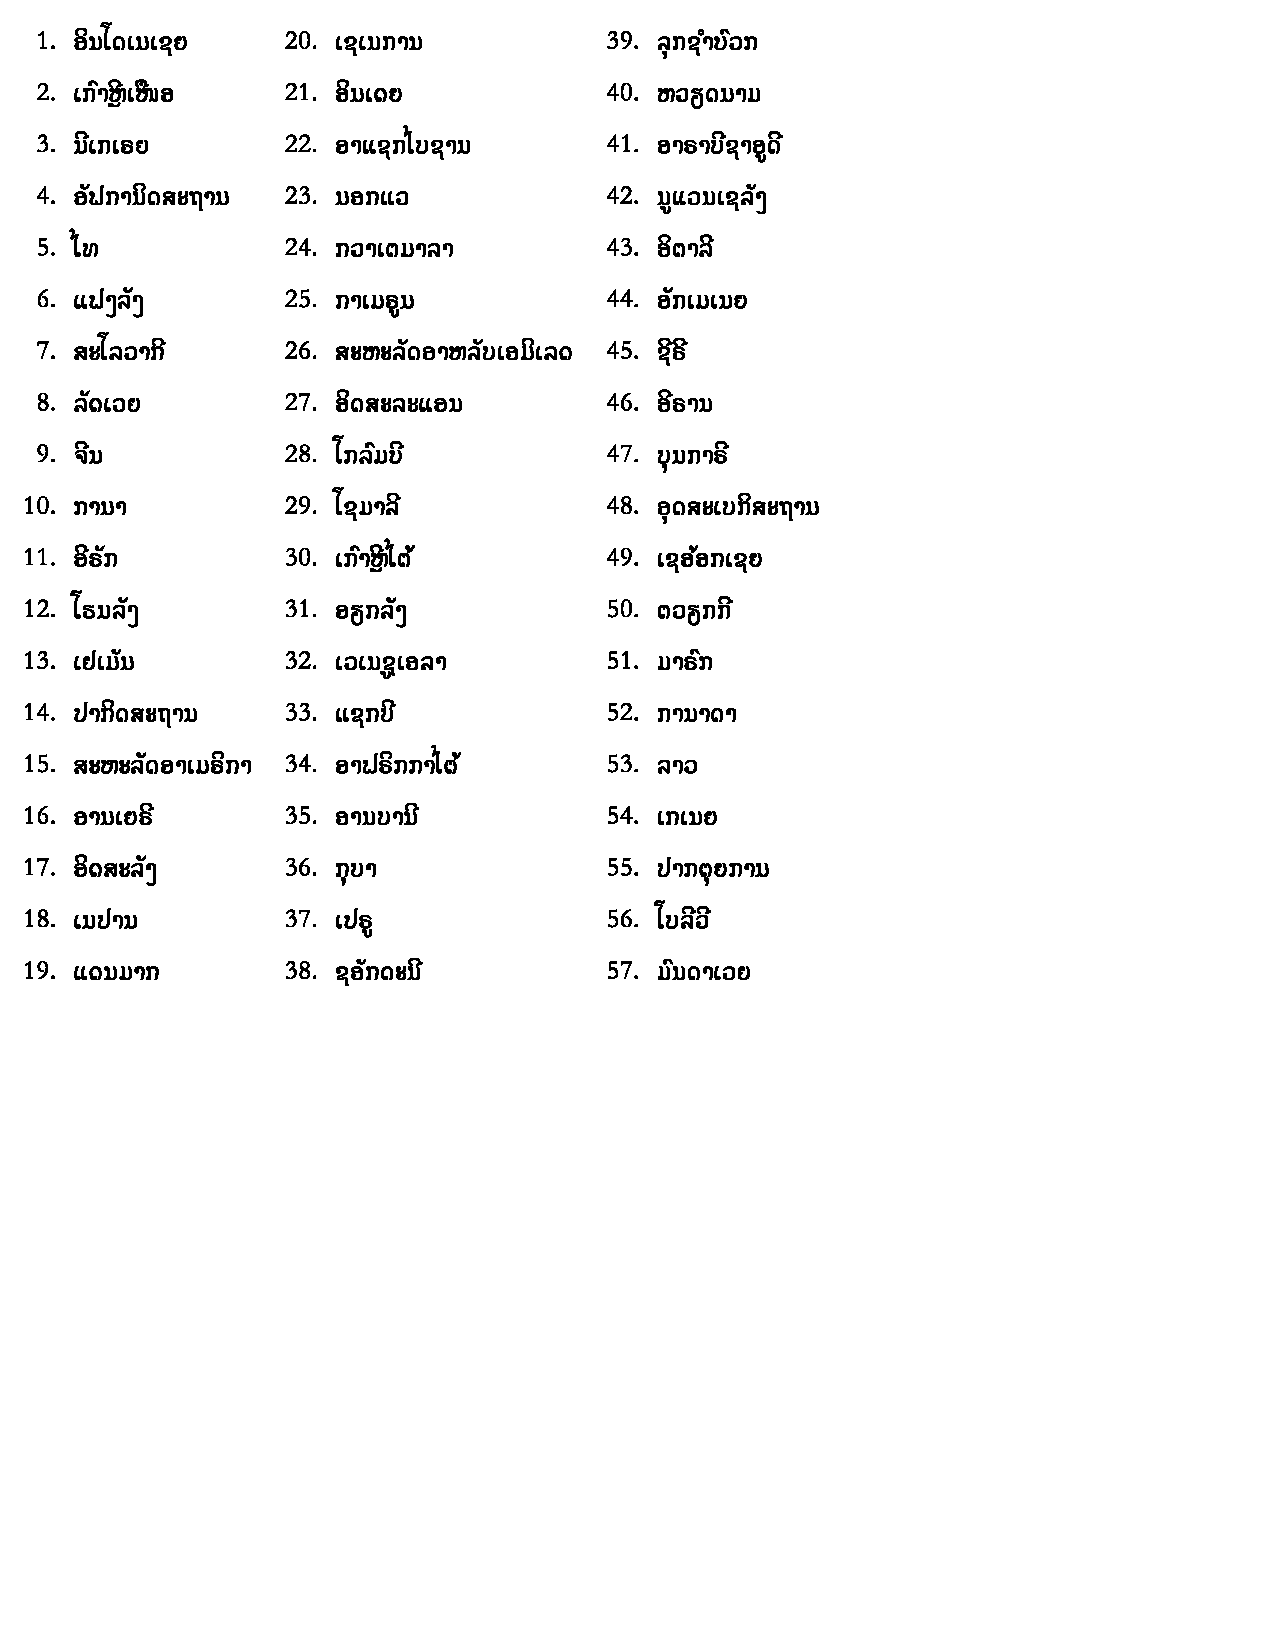
\includegraphics[bb = 0 320 500 800]{geo57Lao.pdf}}

%\makepart{\respsing {\teamcont}}
%\makepart{\solusing {\teamcont}}
%\thispagestyle{empty}
%\pagestyle{somestyle}

%???

\end{document}

